\section{MAVLink Protocol}\label{sec:mavlink}
When speaking of digital communication it is required to have a certain communication protocol. Given the fact that, this project deals with drones, a special protocol, namely Micro Air Vehicle Link (MAVLink) has been taken into consideration. This protocol is used in a GNS and drones scenario, where inter-communication between systems is needed in order to transmit GPS location, heading angle and speed.  

\subsection{Packet Structure}
For further understanding the packet structure of such a protocol is needed as seen in Table \ref{tab:mavlink}.

\begin{table}[h]
	\centering
	\begin{tabular}{|c||c|c|}
		\hline
		Field name       & Index (Bytes)  & Purpose											     \\ \hline\hline
		Start-of-frame   &      0         & Start of frame transmission 							   \\ \hline
		Pay-load-length  &      1         & Length of payload (n)       							   \\ \hline
		Packet sequence  &      2    	  & Sent sequence counter (detect packet loss)                 \\ \hline
		System ID        & 		3		  & Sending system identification 							   \\ \hline
		Component ID     & 		4 		  & Sending component identification 						   \\ \hline
		Message ID       & 		5 		  & Message identification (correctly decoded)      		   \\ \hline
		Payload          &   6 to (n+6)   & Data into the message, depends on Message ID        	   \\ \hline
		CRC              & (n+7) to (n+8) & Check-sum of packet (excluding packet start sign)          \\ \hline
	\end{tabular}
	\caption{MAVLink packet structure}
	\label{tab:mavlink}
\end{table}

The CRC field ensures message integrity of each packet. Another function of the CRC is to establish that both sender and receiver agree on the message transfer. Additionally, a seed value is appended at the end of the data when computing the CRC, generated with every new message.

\subsection{Messages}
As stated above the payload from the packets are MAVLink messages. Also, every message can be identified by its ID field on the packet. Additionally, an XML document (in MAVLink source) has the definition of all the data stored on that payload. A sample of such an XML document can be seen in Figure \ref{fig:mav_msg} which describes a message with an ID 24 giving GPS relevant information.

\begin{figure}[h]
	\centering
	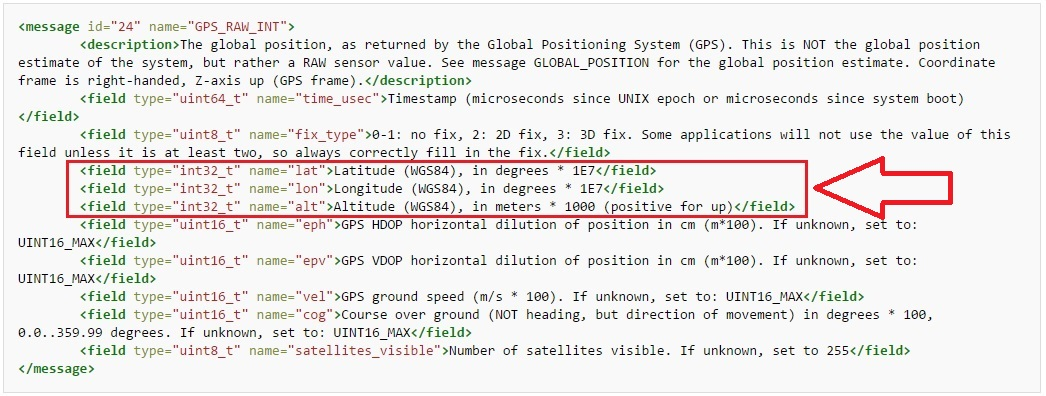
\includegraphics[scale=0.5]{figures/mavlink_msg.jpg}
	\caption{MAVLink message XML document}
	\label{fig:mav_msg}
\end{figure}

To be noted that the XML document describes the logical ordering of the fields for the protocol, not the actual wire format.